\chapter{Machine Learning techniques} \label{chap3}
\section{Introduction}
In this chapter, we will focus on the more traditional methods used in natural language processing such as Naïve-Bayes, decision trees, linear SVM and others. These will serve as baseline for comparing the performances of the more two advanced models that will be analyse later on: LSTM and Attention Mechanism. The first thing to do when working with text is the do words and texts embedding, indeed, in order to use machine learning algorithms on texts, a mathematical representation of these texts is required. 

\section{Text to vectors}
As explained before, text need to be represented in a way that gives more meaningful information than a simple sequence of bits, which have additional drawbacks such that for a given word, the sequence of bits representing it depends on the coding.
 The first and simplest coding that come to mind is a one-hot encoding: a matrix $M$ of size number of texts $\times$ number of words where $M_{ij} = 1$ if the word $j$ is present in the text  $i$ and $0$ in the other case. But this is till not enougth as each word is given the same weight, no matter how often it appears in the text. \\ 

 In order to overcome this problem, term-frequency might be used, that is, rather than setting $M_{ij}$ to 0 or 1 we set it to the number of time it appears in the text. \\ 

 It is possible to use even better text embedding. It is called term-frequency, inverse document frequency. The main idea is that a word that appears often in all the documents is not helpful in order to classify the documents. For example, if the task is to classify books of biology and physics, words atom, cell or light are more useful than today or tomorrow. \\

In order to compute tf-idf, it is separted in two part, the first one being term-frequency and the second one inverse document frequency. We have that \begin{equation}
	tf_{ij} = \#(W_j | W_j \in D_i)\\ 
\end{equation}

That is, $tf_{ij}$ is the number of time the word j appears in the document i. 

Secondly, we have that \begin{equation*}
	idf_{j} = \log(\frac{\#D}{\#(D_i | W_j \in D_i)}) \\
\end{equation*}

This is the log of the total number of documents, over the number of documents that contains the word j.
Finnaly, the value tfidf value is computed by \begin{equation}
	tf-idf_{ij} = tf_{ij} * idf_{j} \\
\end{equation}

This the text embedding methods that will be used in this section. 

\section{Methodology}
\paragraph{} All the methods presented will be tested in tree differents ways: 
\begin{itemize}
	\item On the liar-liar dataset
	\item On the fake corpus dataset, excluding the news from \textit{beforeitsnews.com} and \textit{nytimes.com}
	\item On the fake corpus dataset, including the two pervious domains. 
\end{itemize}

To be more precise, in the first case, the models will be trained on a training set, tunned using validation set and finally tested using test set. In the second case, the same methodology will be used, the dataset have been split be choosing $60\%$ of the text from each domain for training, and $20\%$ for validation and testing. This way have splitting have been choosen because of the uneven representation of each domain in the dataset in order to ensure representation of all the domains in the tree subsets. 

In the last case, the model is trained on all the news but the two domain previously cited and tested on this two domains.  
\subsection{Evaluation metrics}
In order to evaluate each models, multiple evaluation metrics have been used. There are recall, precision and f1-score. It is needed to use multiple metrics because they don't all account for the same values. For instance, it is possible to have a model with a recall of 1 that behave extremely bad because it simply classify all the inputs in the same single class. 

Remember that precision is defined as \begin{equation}
	Precision = \frac{TP}{TP + FP}
\end{equation}

Which means that we can have two different precision, depending on which classes is considered as being positive. This is the proportion of correctly classified positive element over the number of element classified as positive. It is equals to 1 when there is no false positive, but it does not means that all the positive elements are correctly classified as it might be some false negative. The recall helps to solve this problems.

It is defined as \begin{equation}
	recall = \frac{TP}{TP + FN}
\end{equation}

The f1-score combines the recall and the precision. It is defined by 
\begin{equation}
	f1-score = \frac{2 * precision * recall}{precision + recall}\
\end{equation}

It is also possible to look at the weighted average of all these values. For instance, it is possible to compute un global recall be average the recall for both class by the respective class ratio. \\

Finally, raw output can be used by looking at the confusion matrix.\\

The first parameters to tune is the max number of features used by tf-idf. This is the maximum number of words that will be kept to create the text encoding. The words that are kept are the most frequent words. 

\section{Models}
Four models have been used in order to classify texts represented as a TF-IDF matrix. These are Multinomial Naïve-Bayes, Linear SVM, Ridge Classifier and Decision Tree. 
\subsection{Na\"{i}ve-Bayes\cite{zhang_optimality_nodate}}
The basic idea of Naïve-Bayes model is that all features are independent of each other. This is a particulary strong hypotheses in the case of text classification because it suppose that words are not related to each others. But it know to work well given this hypotheses. 

Given an element of class y and vector of feature $\mathbf{X} = (x_1,...,x_n)$. The probability of the class given that vector is defined as 
\begin{equation}
	P(y | \mathbf{X}) = \frac{P(y)*P(\mathbf{X} | y)}{P(\mathbf{X})}
\end{equation}

Thanks to the assumption of conditional independance we have that 

\begin{equation}
	P(x_i |y,x_1, ...,x_{i-1},x_{i+1},...,x_n) = P(x_i | y)
\end{equation}
Using bayes rules we have that
\begin{equation}
	P(y|x_1,...,x_n) = \frac{P(y)\prod_{i=1}^n P(x_i | y)}{P(x_1,...,x_n)}
\end{equation}

Because $P(x_1,...,x_n)$ is constant, we have the classification rule 
\begin{equation}
	\hat{y} = \underset{y}{argmax} P(y)\prod_{i=1}^n P(x_i | y)
\end{equation}

\subsection{Linear SVM}
Linear SVM is a method for large linear classification. Given pairs of features-label $(\mathbf{x_i}, y_i), y_i \in \{-1, 1\}$, it solve the following unconstrained optimization problem. 
\begin{equation}
	\underset{w}{min} \frac{1}{2} \mathbf{w^Tw} + \mathbf{C} \sum_{i=1}^l \xi(\mathbf{w;x_i},y_u)
\end{equation}

Where $\xi$ is a loss function, in this case L2 loss function have been used, and $\mathbf{C} > 0$ a pennality parameter. 

Class of new examples are assigned by looking at the value of $\mathbf{w^Tw}$. The class 1 is assigned if $\mathbf{w^Tw} \geq 0$ and the class $-1$ if $\mathbf{w^Tw} < 0$.

\subsection{Decision Tree}
\subsection{Ridge Classifier}
Ridge classifier works the same way as ridge regression. It states the problem as a minimization of the sum of square errors with penalization. It can be expressed as in \textbf{Equation \ref{eq:ridge}}.
\begin{equation}
	\underset{w}{min} ||Xw-y||^2_2 + \alpha ||w||^2_2 \label{eq:ridge}
\end{equation}
The predicted class if positive if Xw is positive and negative otherwise. 
\section{Models on liar-liar dataset}
\subsection{Linear SVC}
In the case of linear SVC there is one parameters to tune up, which is the penality parameters for the error term. \textbf{Figure \ref{fig:chap3:linearSVC}} show the tree main metrics with respect to the panlity parameter. This show that a parameters of around $0.1$ is the best one. 

\begin{figure*}[]
	\centering
	\makebox[\textwidth][c]{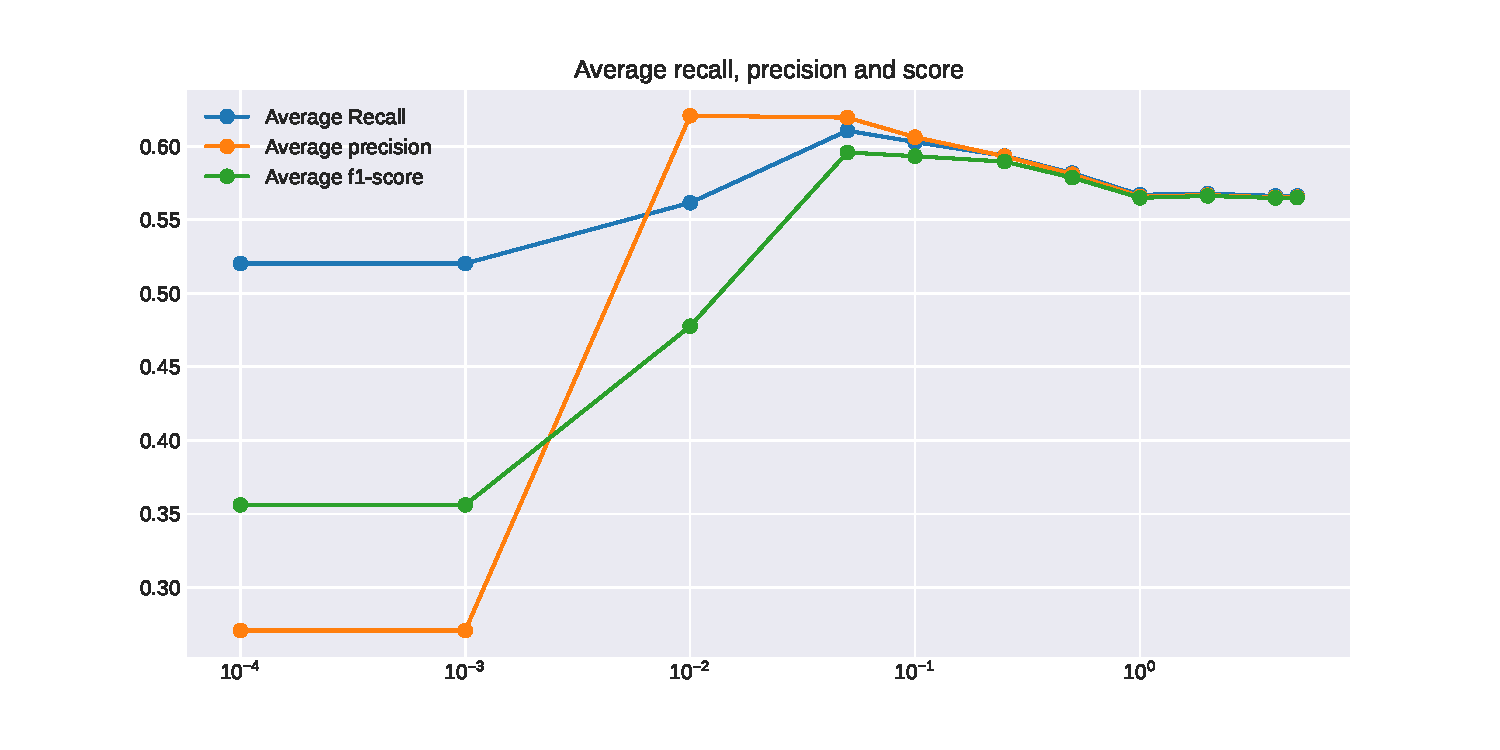
\includegraphics[width=1\textwidth]{images/chapitre3/svc_liar.pdf}}
	\caption{Tuning linearSVC parameters }
	\label{fig:chap3:linearSVC}
\end{figure*}

\subsection{Decision Tree}
With decision tree, it is possible to reduce overfitting by pruning the tree. It is possible to do preprunning or post pruning. Pre pre preuning means that a stoping criterion is used to stop tree growth earlier and post pruning cut the tree once it have been fully grown. It this case pre pruning is done by limiting the maximum depth of the tree. 

\begin{figure*}[]
	\centering
	\makebox[\textwidth][c]{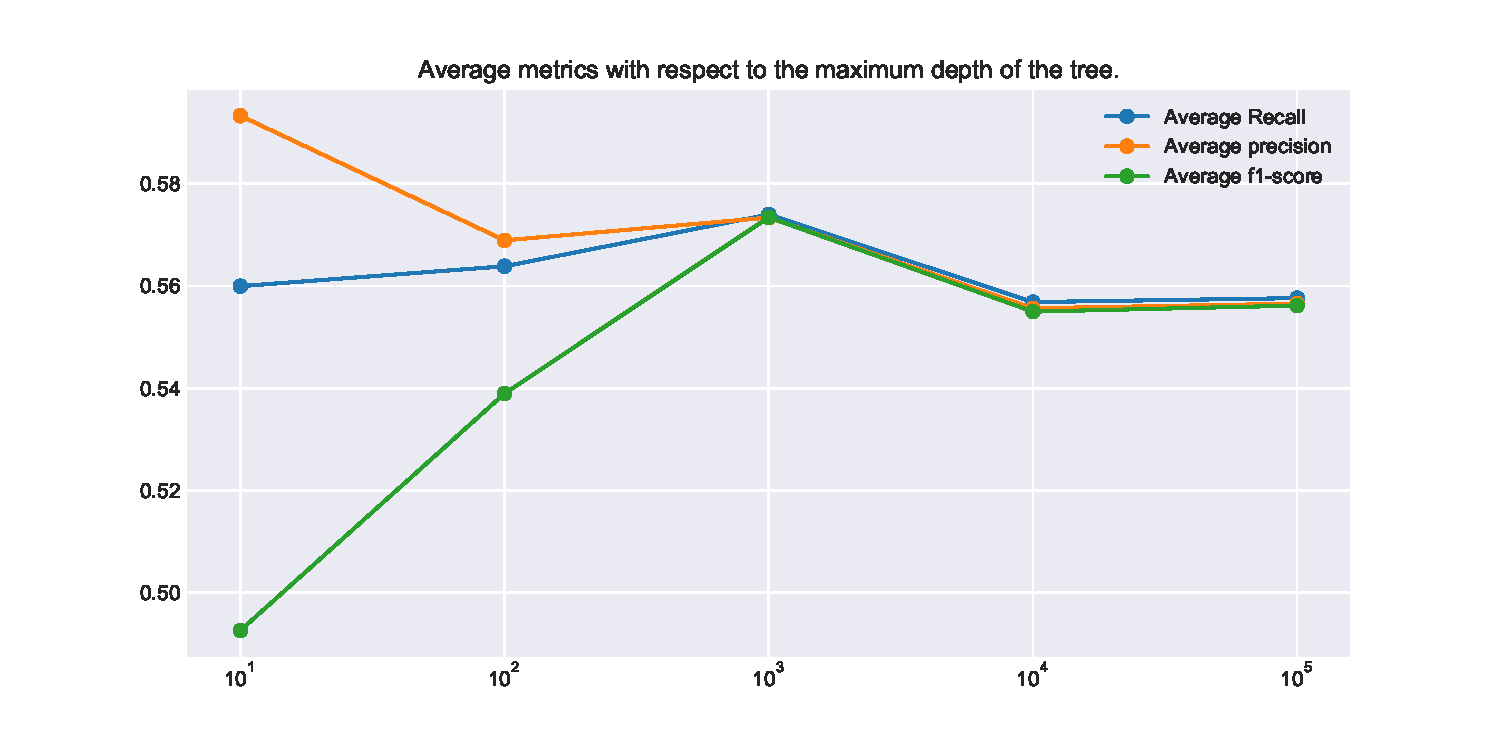
\includegraphics[width=1\textwidth]{images/chapitre3/liar-dt.pdf}}
	\caption{Tuning decision tree parameters }
	\label{fig:chap3:dt}
\end{figure*}

\textbf{Figure \ref{fig:chap3:dt}} shows metrics values for different depths. It seems that tree of depth 1000 are the best ones.
\subsection{Ridge Classifier}
With the ridge classifier model it is also possible to tweak the pennality value of the optimization problem. At \textbf{Figure \ref{fig:chap3:ridge1}} we can see that the optimal parameter is around 10 or 20, depending of the metrics that we want to maximize. Later on, the value of 10 will be chose as a comprimse between precision and recall. It is the value that maximize the f1-score. 

\begin{figure*}
	\centering
	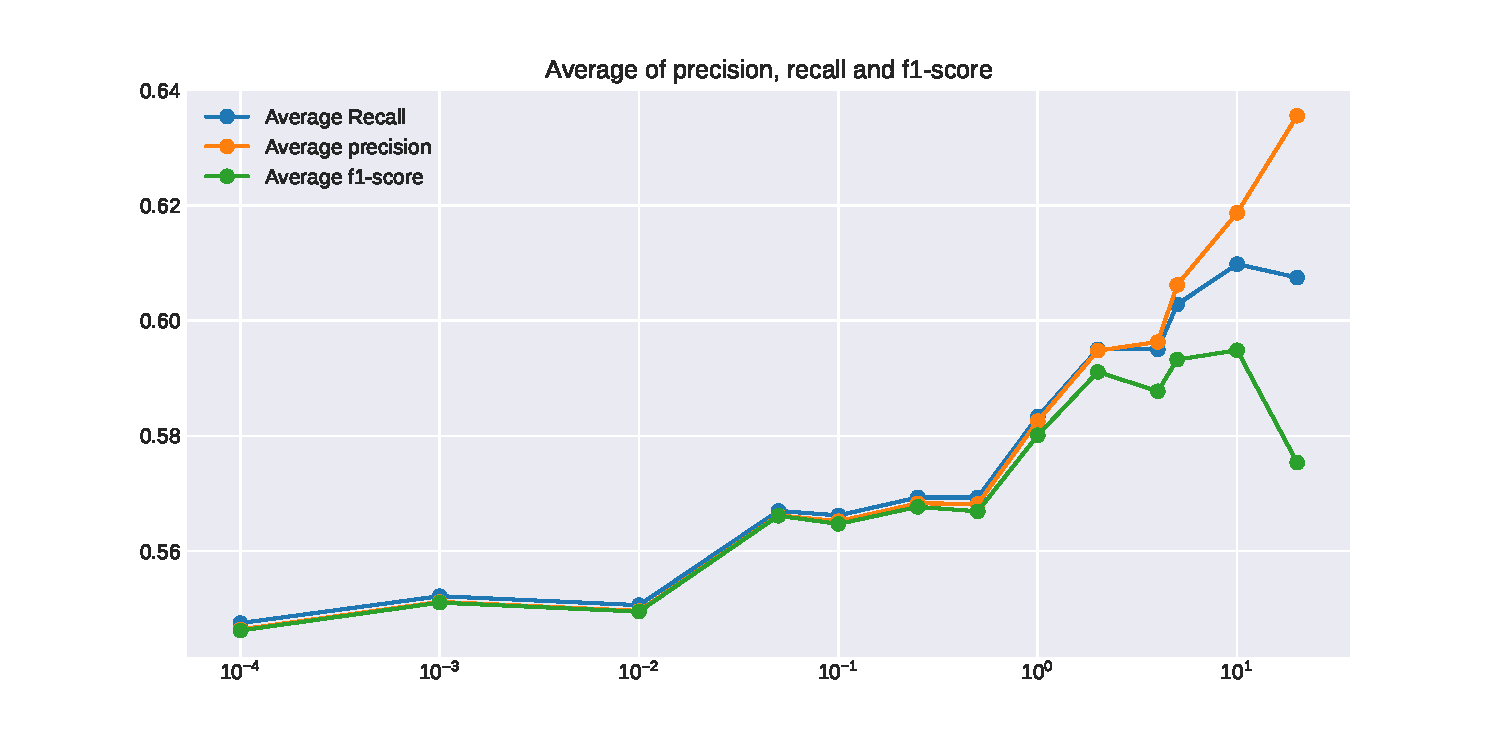
\includegraphics[width=1\textwidth]{images/chapitre3/liar-ridge}
	\caption{Average metrics for ridge classifier with respect to the penality parameter.}
	\label{fig:chap3:ridge1}
\end{figure*} 
\subsection{Max Feature Number}

Starting with the maximum number of features, the precision of each model can be analyzed when limiting the maxium number of words. The results for each model can be seen at \textbf{Figure \ref{fig:chap3:max_feature3}, \ref{fig:chap3:max_feature1}} and \textbf{\ref{fig:chap3:max_feature2}}. Shows that depending on the metrics we want to optimize it is better to choose different parameters. For instance, in order to maximize F1-score, it is better to use a maximum number of features of 1000.\\

The results are slightly different if the goal is to optimize the precision because if the best value stay the same for Linear SVM and Ridge Classifier, the Naïve-Bayes works better when using the maxium number of features and it goes the same way for recall. 
Based on \textbf{Figure \ref{fig:chap3:max_feature3}} we can say that when it comes to precision and recall, Naïve-Bayes is the one that perform the best.\\

Row results for max features selection are available at \textbf{Appendix \ref{Appendix1}}.
\begin{figure*}[]
	\centering
	\makebox[\textwidth][c]{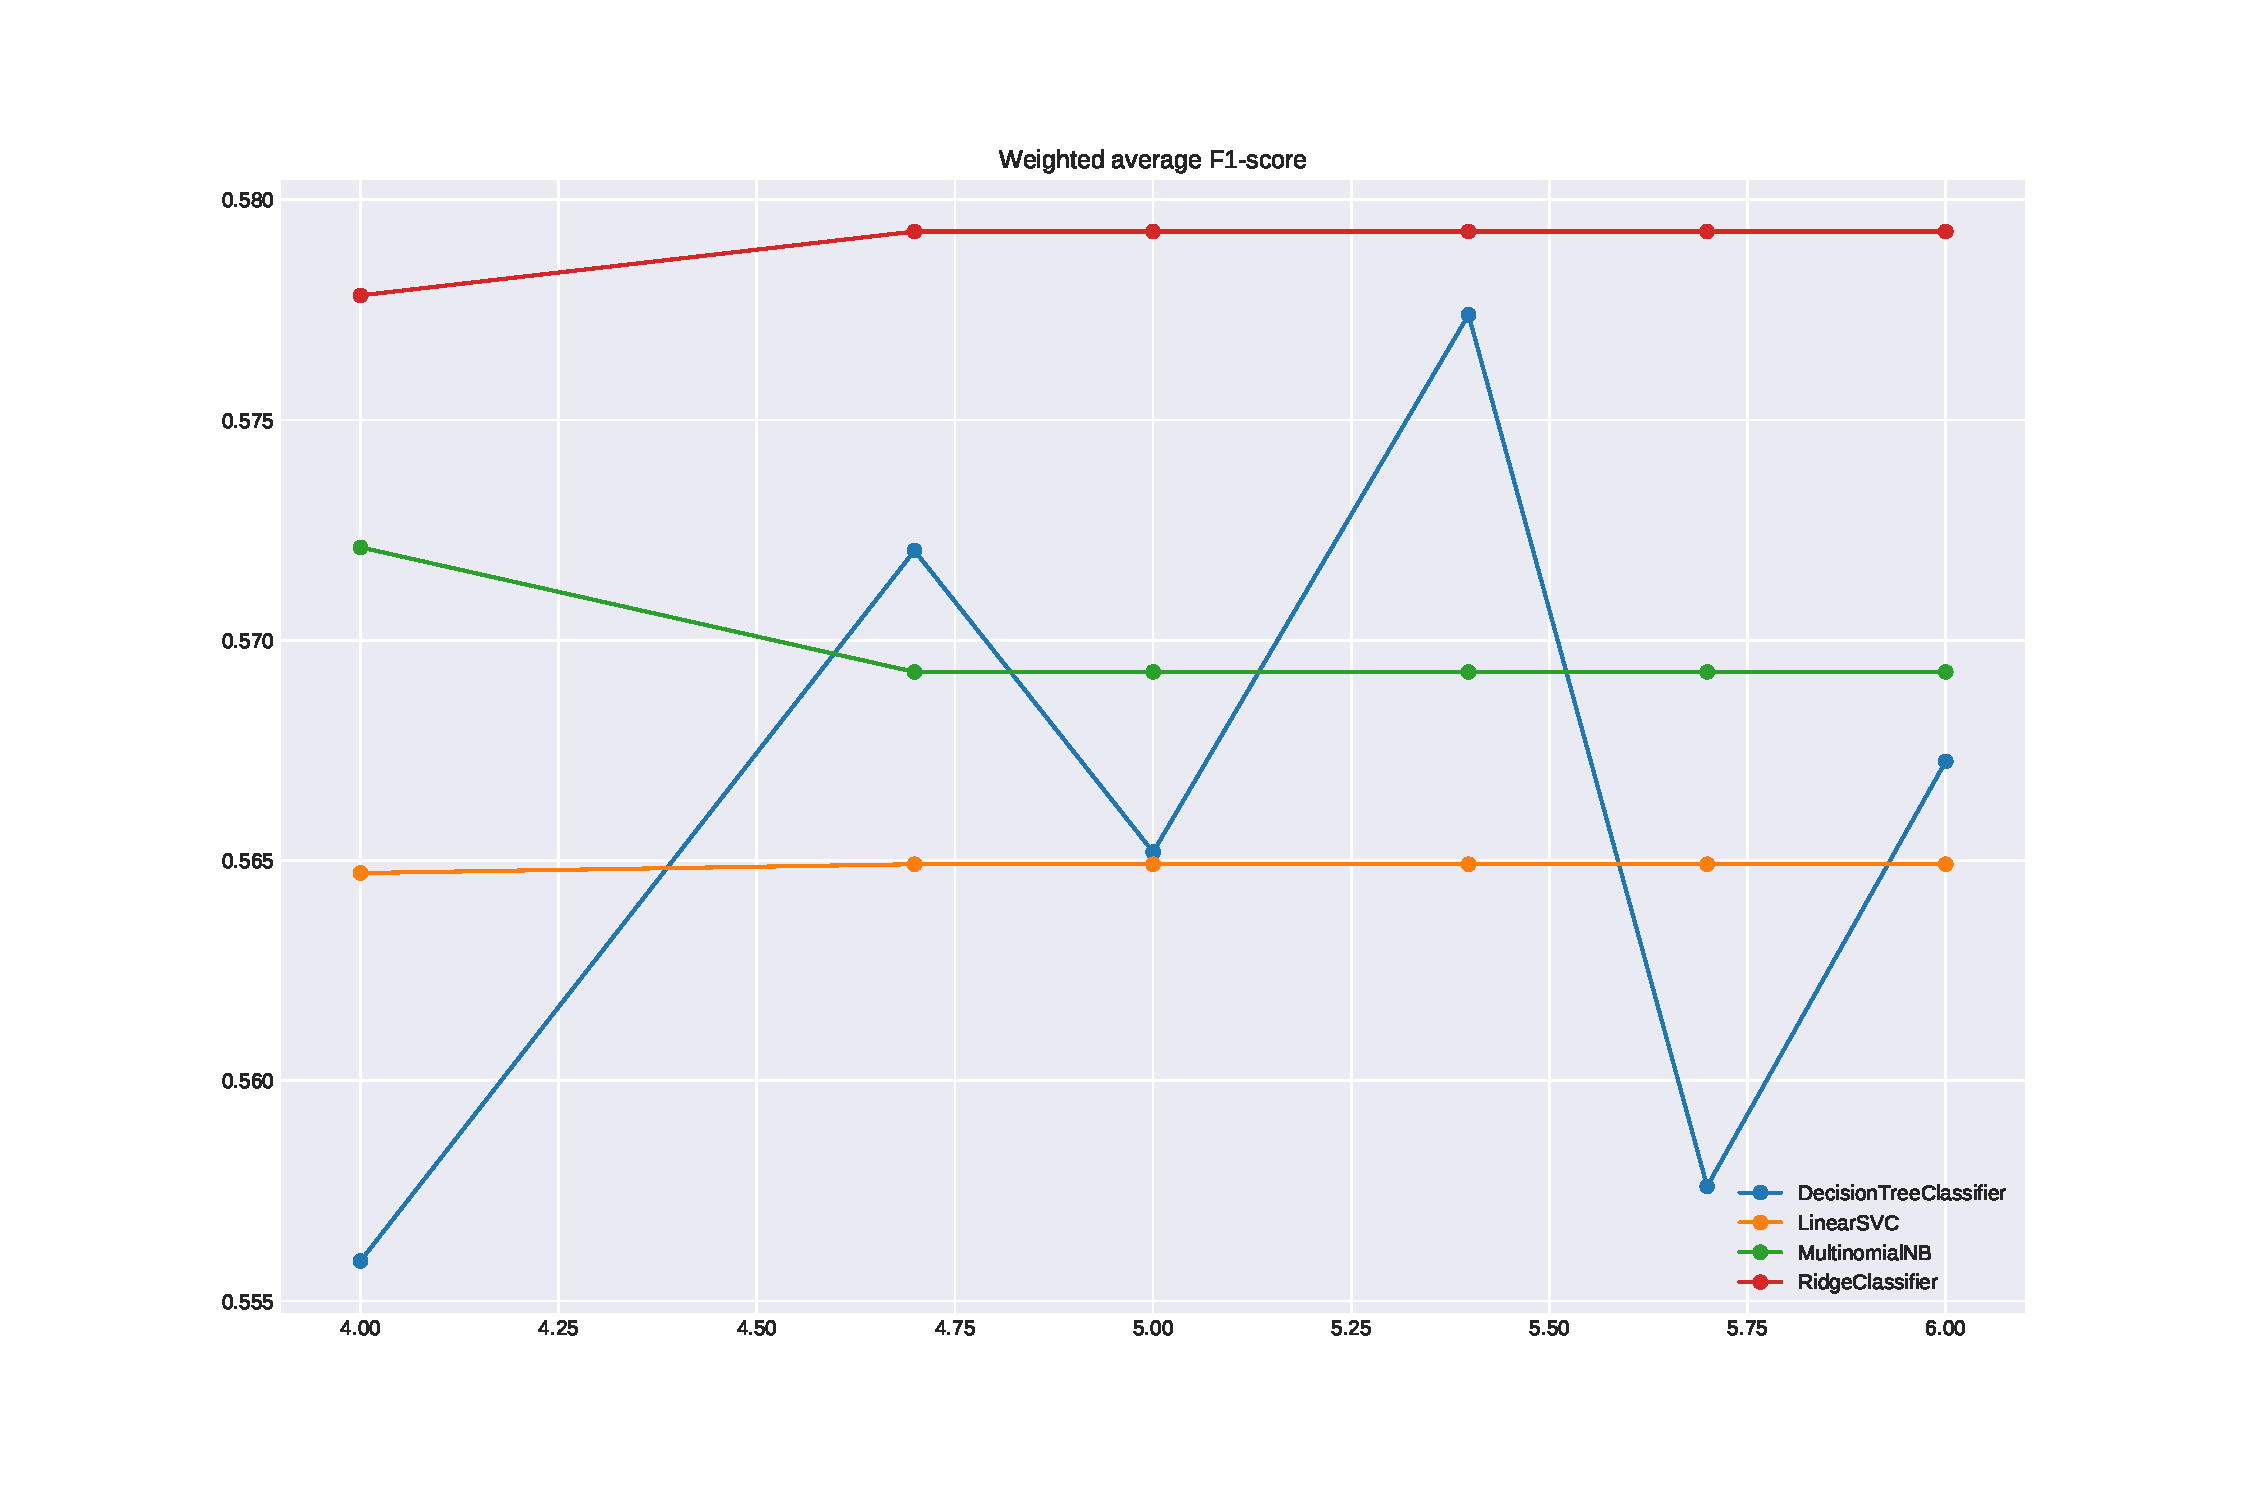
\includegraphics[width=1.2\textwidth]{images/chapitre3/liar-liar_f1_ML}}
	\caption{Weigted average of f1-score, precision and recall of each classes. }
	\label{fig:chap3:max_feature3}
\end{figure*}
It goes differently when we focus on a single class. For example, the precision for fake detection is at its maxium for Linear SVM and Ridge Classifier when only 10 features are used. But at the same time, it is at its minium for reliable class. Its shows that when trying to optimze the overall model and not only for a single class, it is better to look at the weighted average than at the value for a single clas. But it is still important to look at the metrics for a single class because it indicate how it behave for this class. For instance, in the case of automatic fake news detection, it is important to minimize the number of reliable news missclassified in order to avoid what could be called censorship. 
\begin{figure*}[]
	\centering
	\makebox[\textwidth][c]{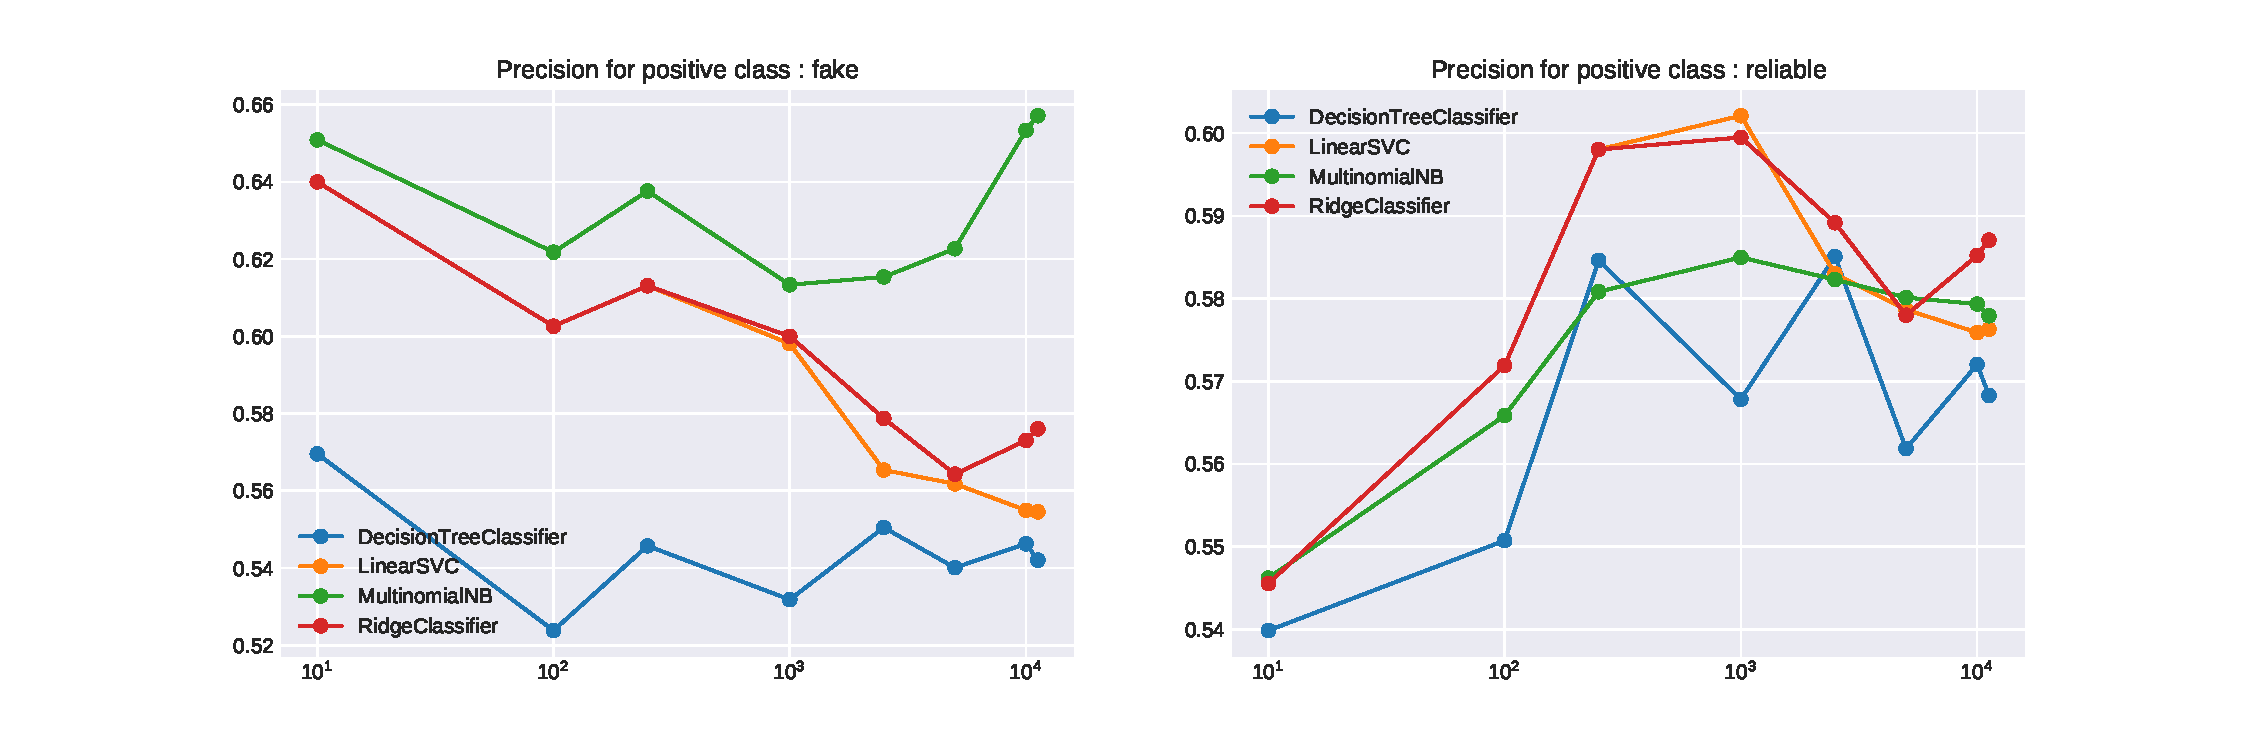
\includegraphics[width=1.2\textwidth]{images/chapitre3/liar-liar_precision_ML}}
	\caption{Precision of the model for each classes, the x axes is log scale of the number of features}
	\label{fig:chap3:max_feature1}
\end{figure*}

\begin{figure*}[]
	\centering
	\makebox[\textwidth][c]{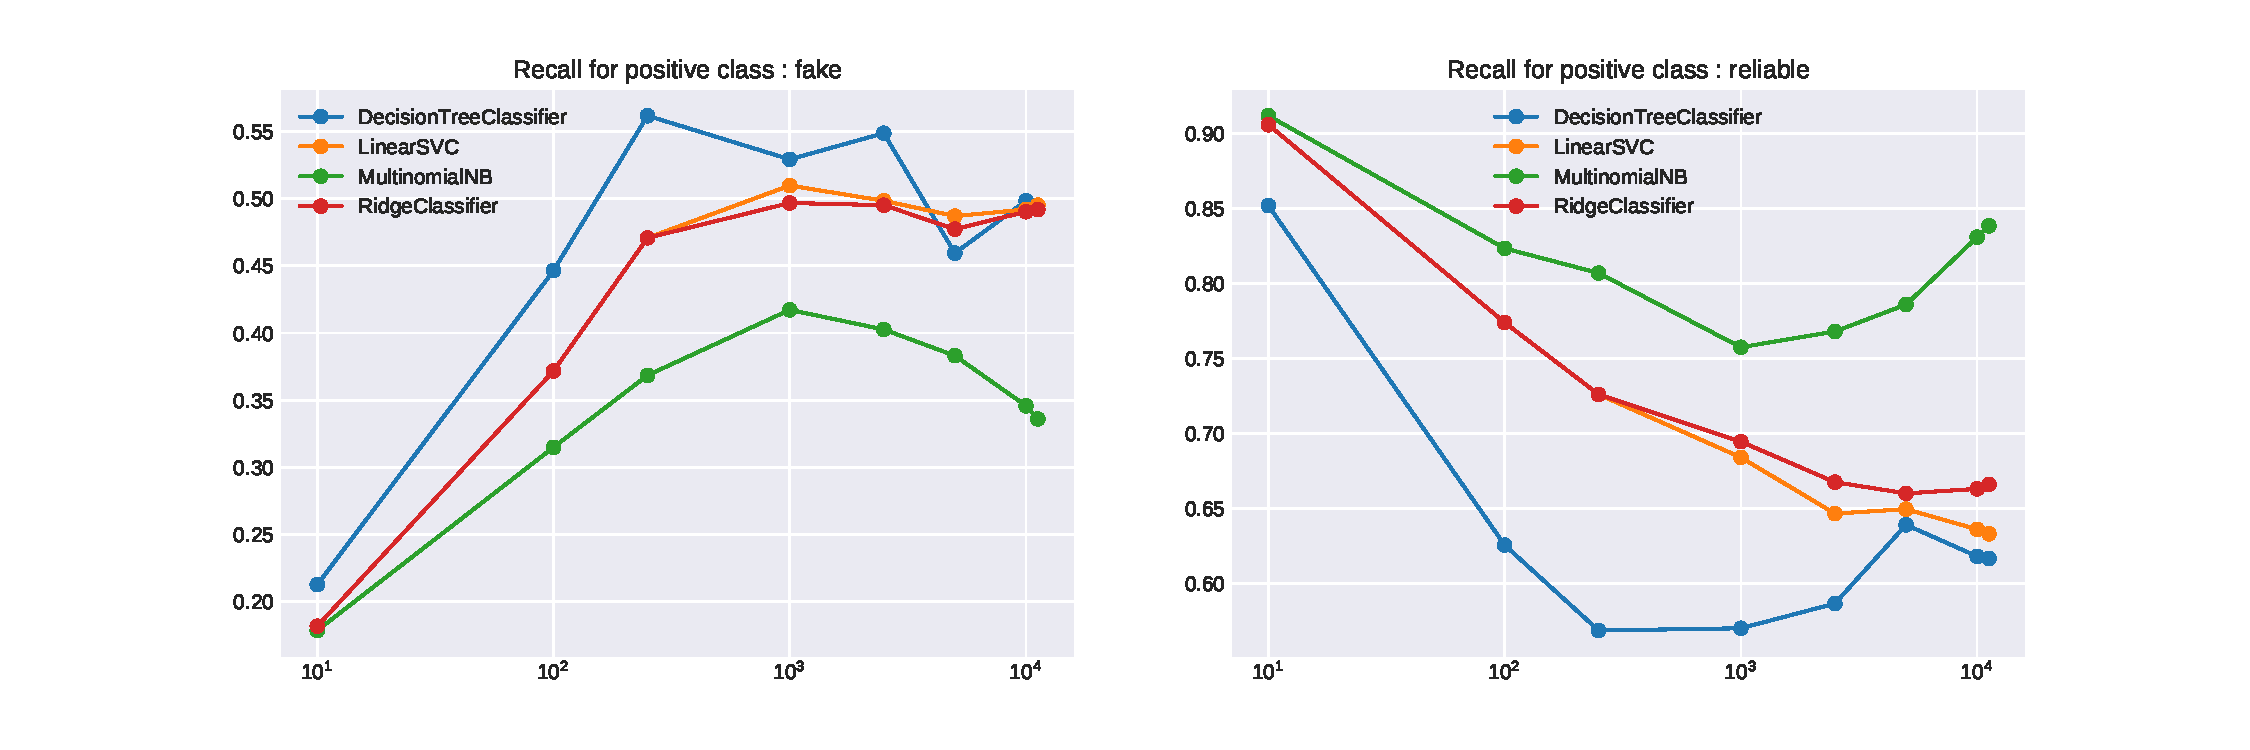
\includegraphics[width=1.2\textwidth]{images/chapitre3/liar-liar_recall_ML}}
	\caption{Precision of the model for each classes, the x axes is log scale of the number of features}
	\label{fig:chap3:max_feature2}
\end{figure*}

\section{Models on fake corpus dataset}
\subsection{SMOTE: Synthetic Minority Over-sampling Technique\cite{Chawla2011}}
As it have been show in \textbf{Chapter \ref{chap2}}, the fake news corpus is inbalanced. Synthetic minority over-sampling is a technique that allows to generate fake samples from the minor class. It works by randomly choosing one or many neirest neigbhor in the minority class. For instance, if the algorithm is set to use 5 nearest neigbours, for each samples it will choose one of its nearest neigbours, and generate a new sample on the segment joining the sample and its neigbour. 

\begin{algorithm}
	 \KwData{k = Number of nearest neighbors}
	 \KwData{T = number of minority class samples}
	 \For{$i \leftarrow 1...T$}{Compute k-nearest neighbors of sample i\;
	 	Populate(knn, i)\;}
	 \caption{SMOTE}
	 \label{algo:SMOTE}
\end{algorithm}

\begin{algorithm}
	\KwData{knn = the k nearest neighbour of sample i}
	\KwData{s = ith sample}
	nn = random\_choice(knn)\;
	newSample = s + rand(0, 1) * (nn - s)\;
	\caption{Populate}
	\label{algo:populate}
\end{algorithm}

\textbf{Algorithm \ref{algo:SMOTE}} and \textbf{\ref{algo:populate}} shows how it works. The first one compute the k-nearest neighbors and the second one compute a new element by randomly choosing one of this neighbors. 

\subsection{Results without using SMOTE}
\subsubsection{Hyperparameters tuning}
As for the models trained on the \textbf{liar-liar corpus}, hyper-parameters can be optimized the same way. The average metrics for each models with respect to there paramters are shown at \textbf{Figure \ref{fig:chap3:ridge2}, \ref{fig:chap3:dt2}} and \textbf{\ref{fig:chap3:lsvm2}}. \\

\begin{figure*}
	\centering
	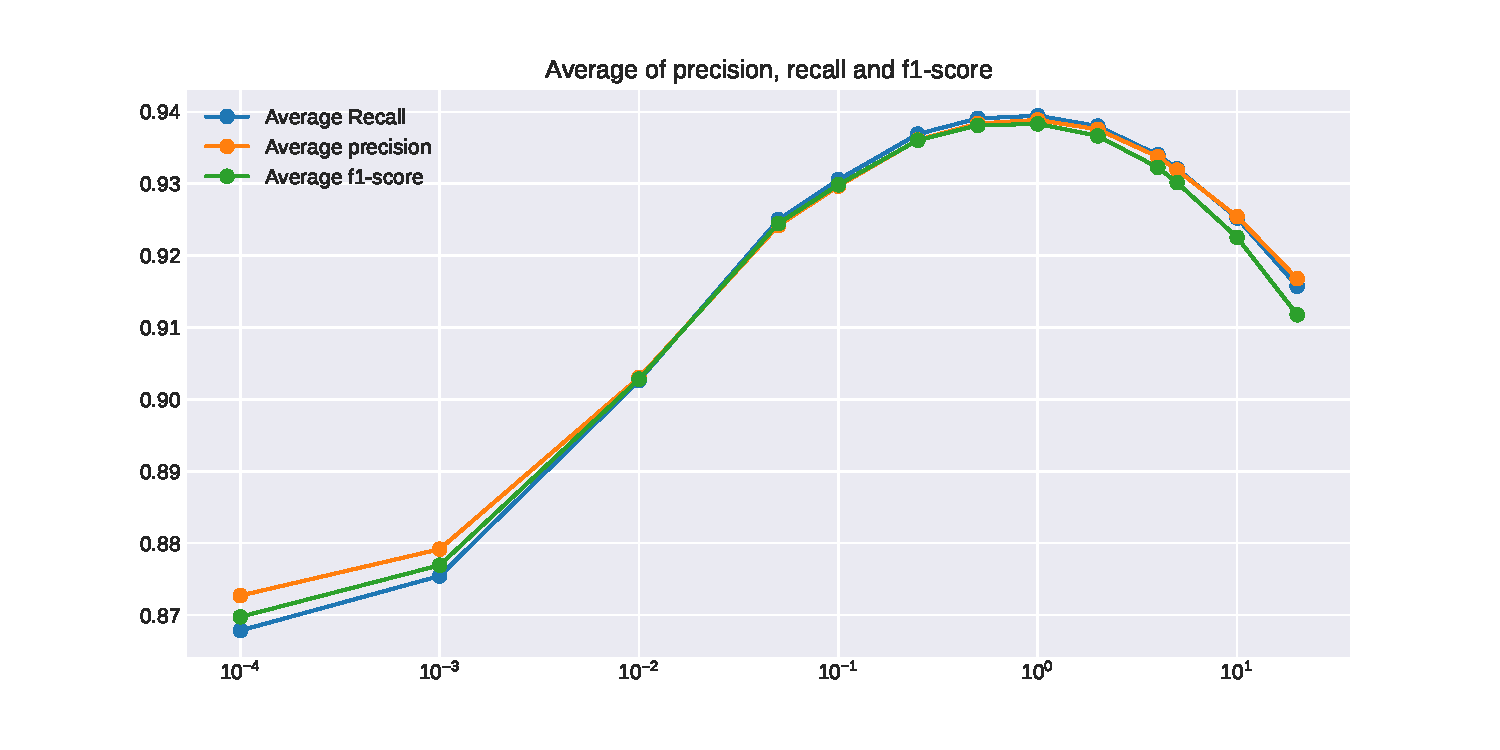
\includegraphics[width=0.8\textwidth]{images/chapitre3/ridge}
	\caption{Metrics value with respect to the penality paramter for ridge classifier}
	\label{fig:chap3:ridge2}
\end{figure*}
The optimal parameter for the ridge classifier is clearly 1. As well as for the decision tree trained on \textbf{liar-liar} dataset, the optimal maximum depth is of 1000. 
\begin{figure*}
	\centering
	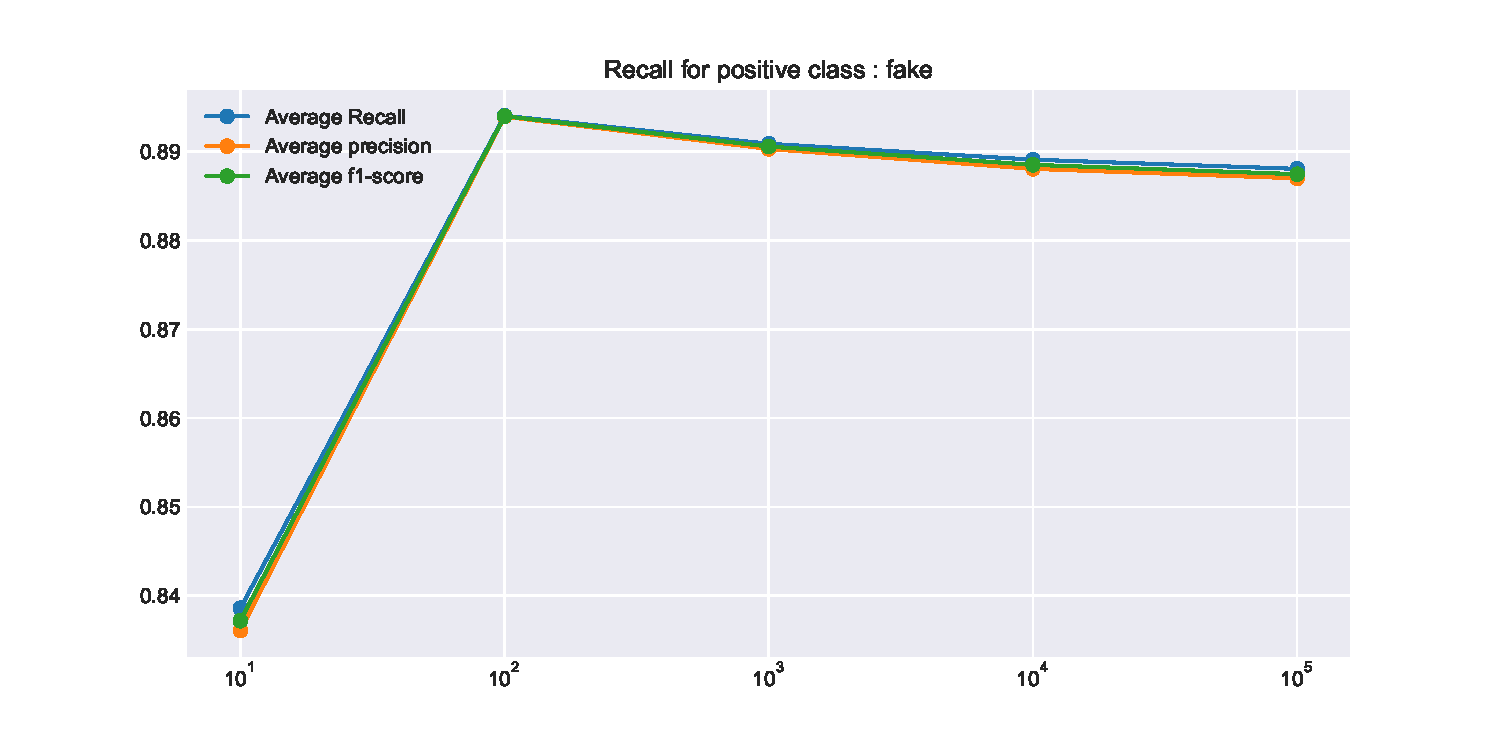
\includegraphics[width=0.8\textwidth]{images/chapitre3/fake-dt}
	\caption{Optimal depth of decision tree.}
	\label{fig:chap3:dt2}
\end{figure*}
And finaly, the optimal value for the penality parameter of the svm is also 1.\\
\begin{figure*}
	\centering
	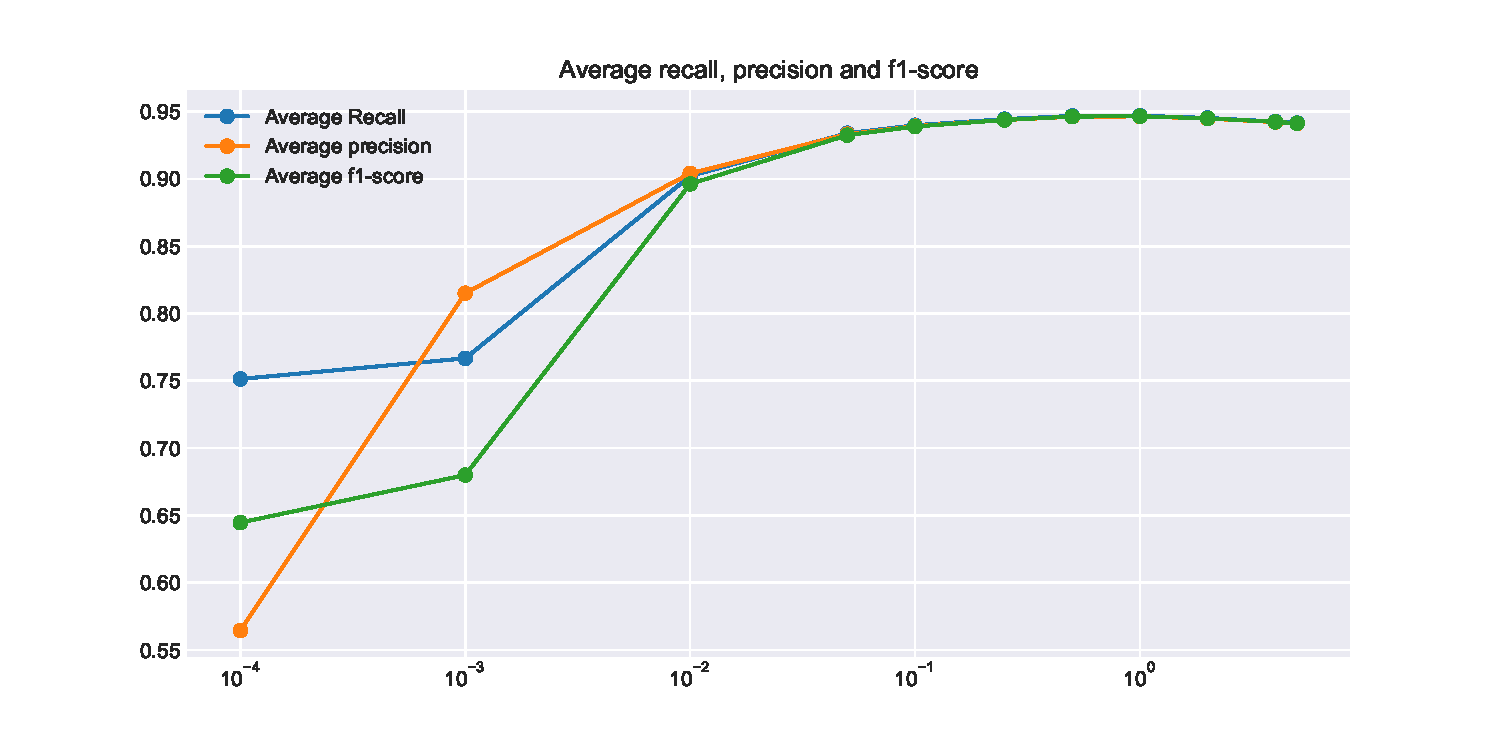
\includegraphics[width=0.8\textwidth]{images/chapitre3/svc_fake}
	\caption{Optimal penality parameters for linear svm}
	\label{fig:chap3:lsvm2}
\end{figure*}

By looking at \textbf{Figure \ref{fig:chap3:max_feature1}, \ref{fig:chap3:max_feature2}} and \textbf{\ref{fig:chap3:max_feature3}} we can find optimal parameters for the number of features used in TF-IDF. It shows that linear svm and ridge classifier are the ones that perform the best, having an average precision of sligtly more than $94\%$ for the linear svm and $94\%$ for the ridge classifier. They acheive these performances from $50,000$ features and does not decrease. On the other hand, Naïve-Bayes reches a pike at $100,000$ features and greatly decrease afterward. \\

\begin{figure*}
	\centering
	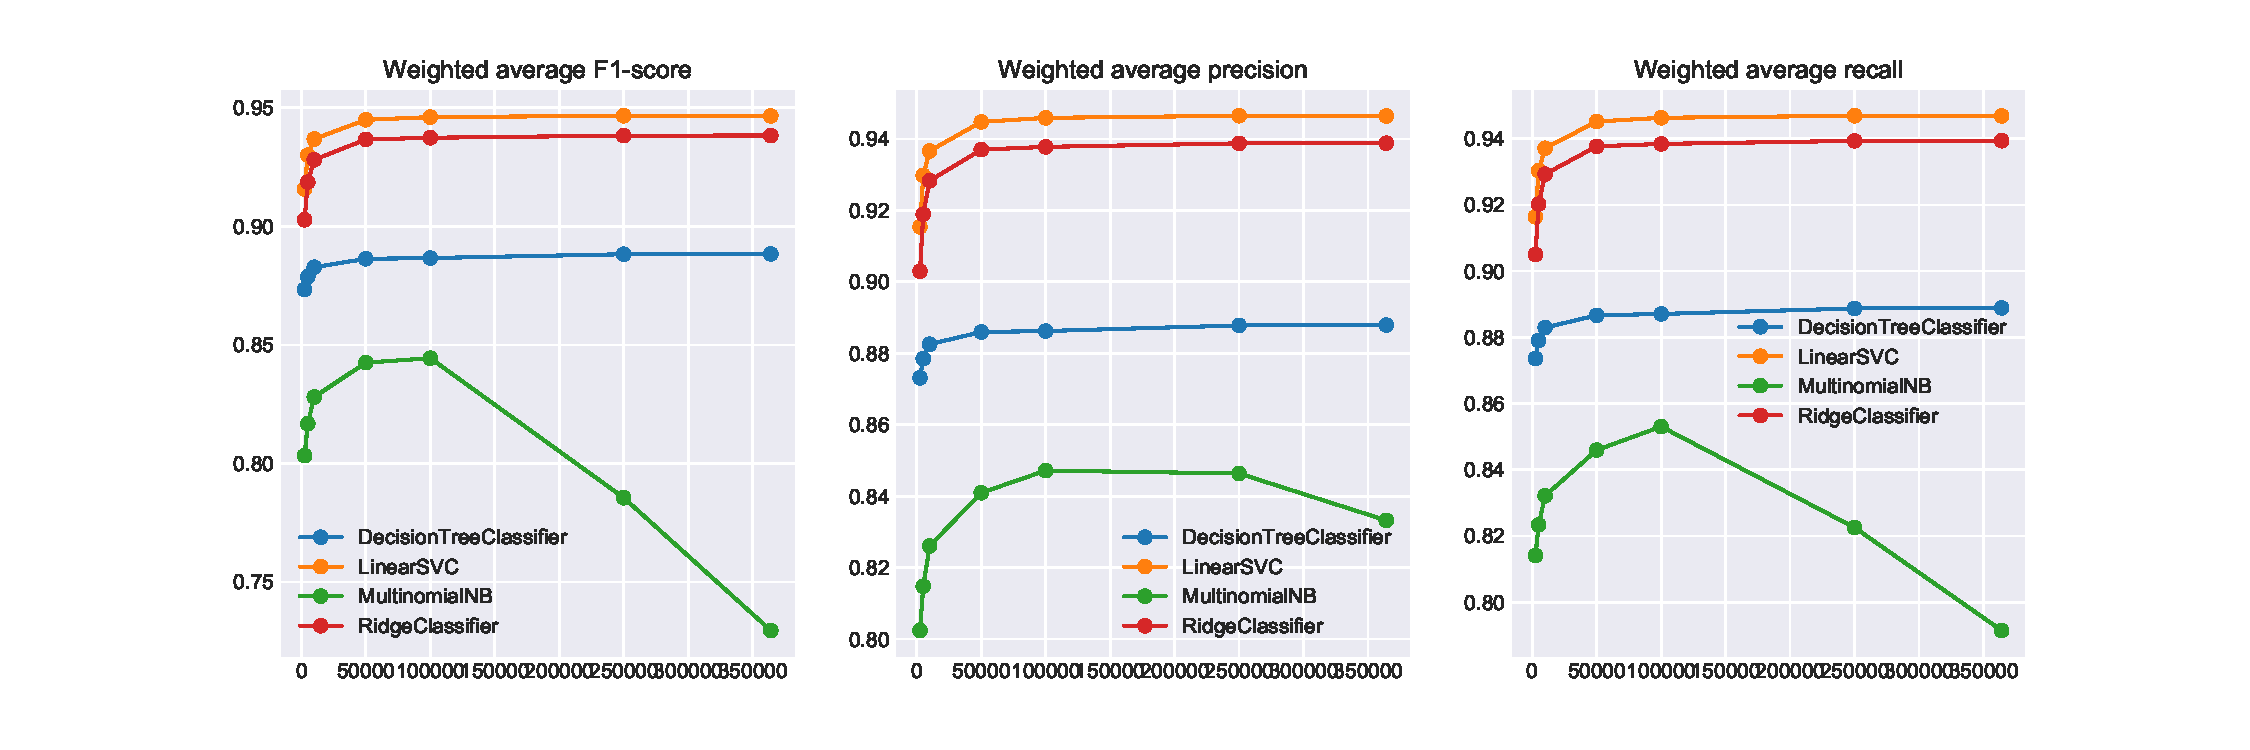
\includegraphics[width=0.8\textwidth]{images/chapitre3/ML_fake_average}
	\caption{Average recall, precision and f1-score wti respect to the maxiumum number of features.}
	\label{fig:chap3:max_feat1}
\end{figure*}
\begin{figure*}
	\centering
	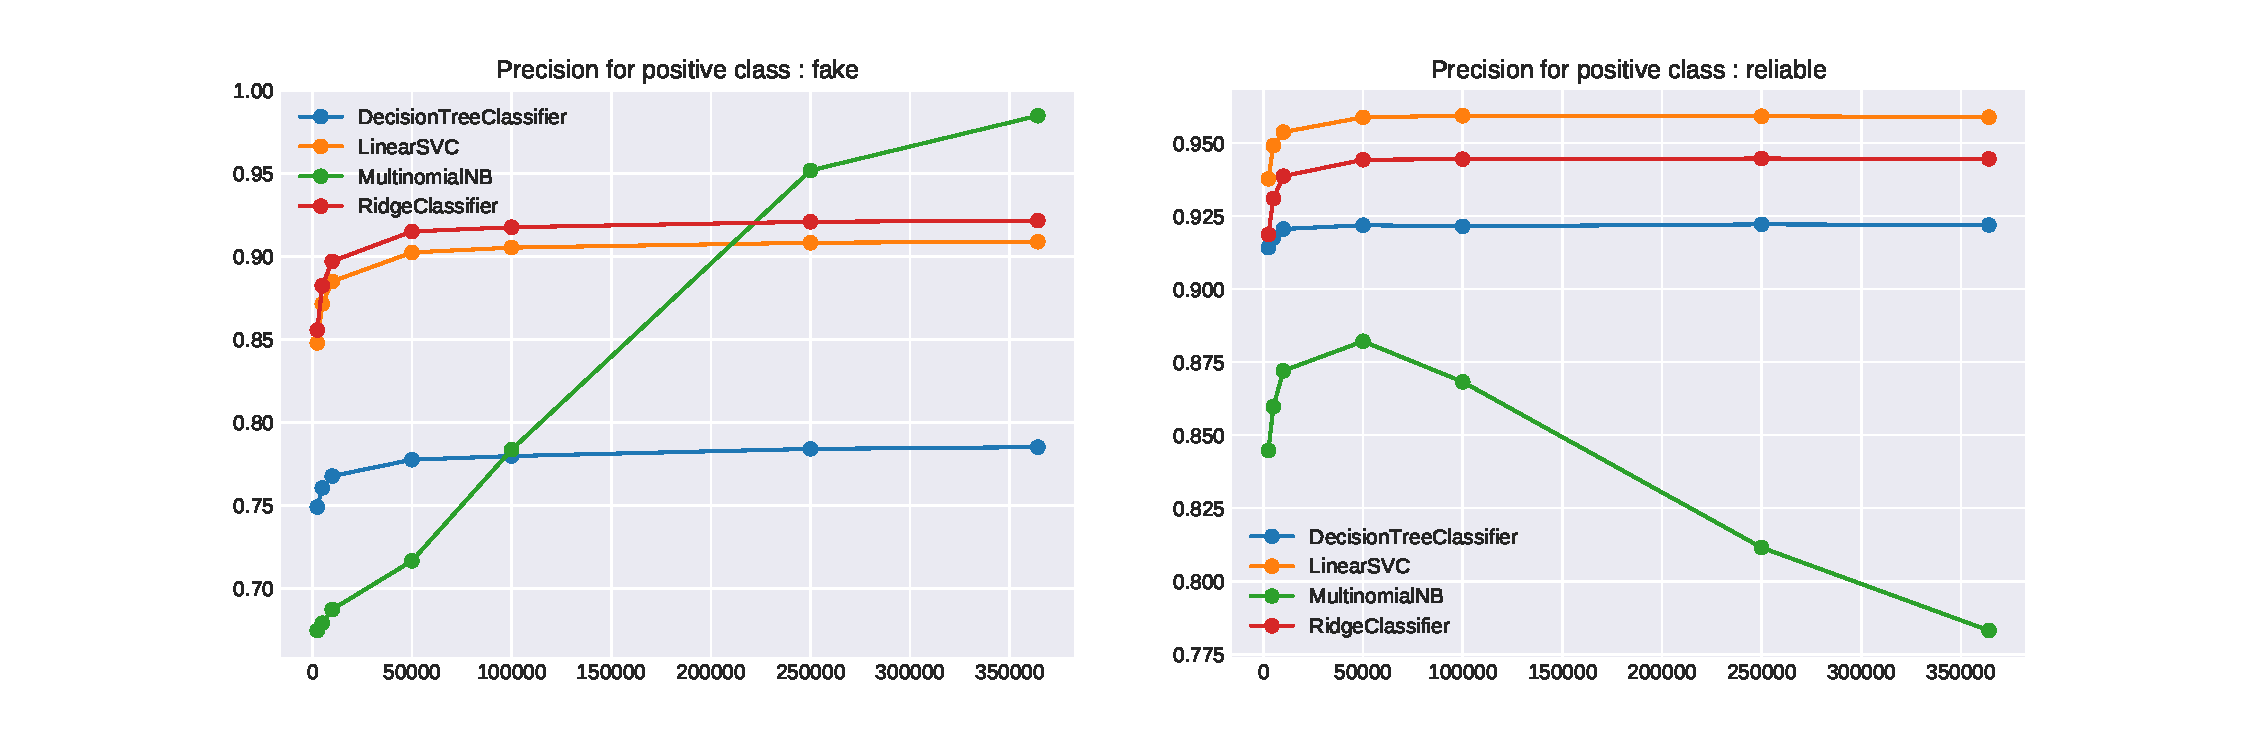
\includegraphics[width=0.8\textwidth]{images/chapitre3/ML_fake_precision}
	\caption{Precision for fake and reliable class for each model with respect to the maxiumum number of features}
	\label{fig:chap3:max_feat2}
\end{figure*}
\begin{figure*}
	\centering
	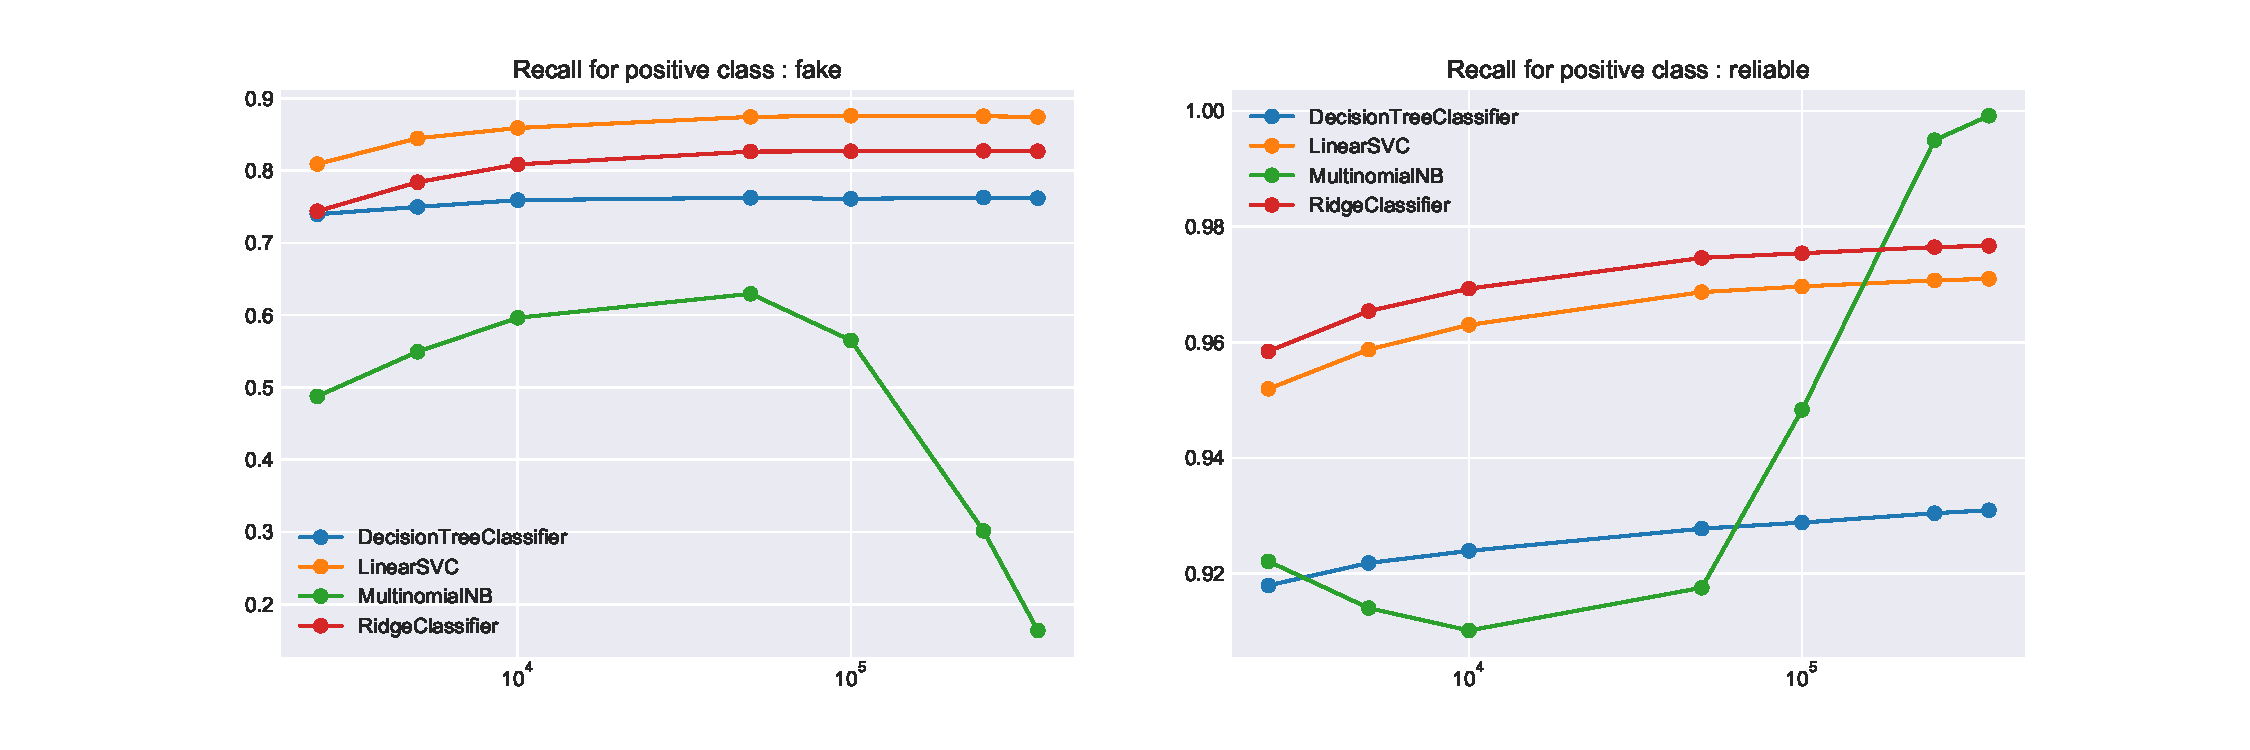
\includegraphics[width=0.8\textwidth]{images/chapitre3/ML_fake_recall}
	\caption{Recall for fake and reliable class for each model with respect to the maxiumum number of features}
	\label{fig:chap3:max_feat3}
\end{figure*}


\textbf{Figure \ref{fig:chap3:max_feature3}} shows why it is important to look at all the metrics, because Naïve-Bayes reaches a recall of 1 for the reliable class and close to 0 for the fake class, which means that almost all the text are classified as reliable. This can be verified by looking at \textbf{Figure \ref{fig:chap3:confMat1}}, only a small proportion of true fake are actualy classified as it.

\begin{figure*}
	\centering
	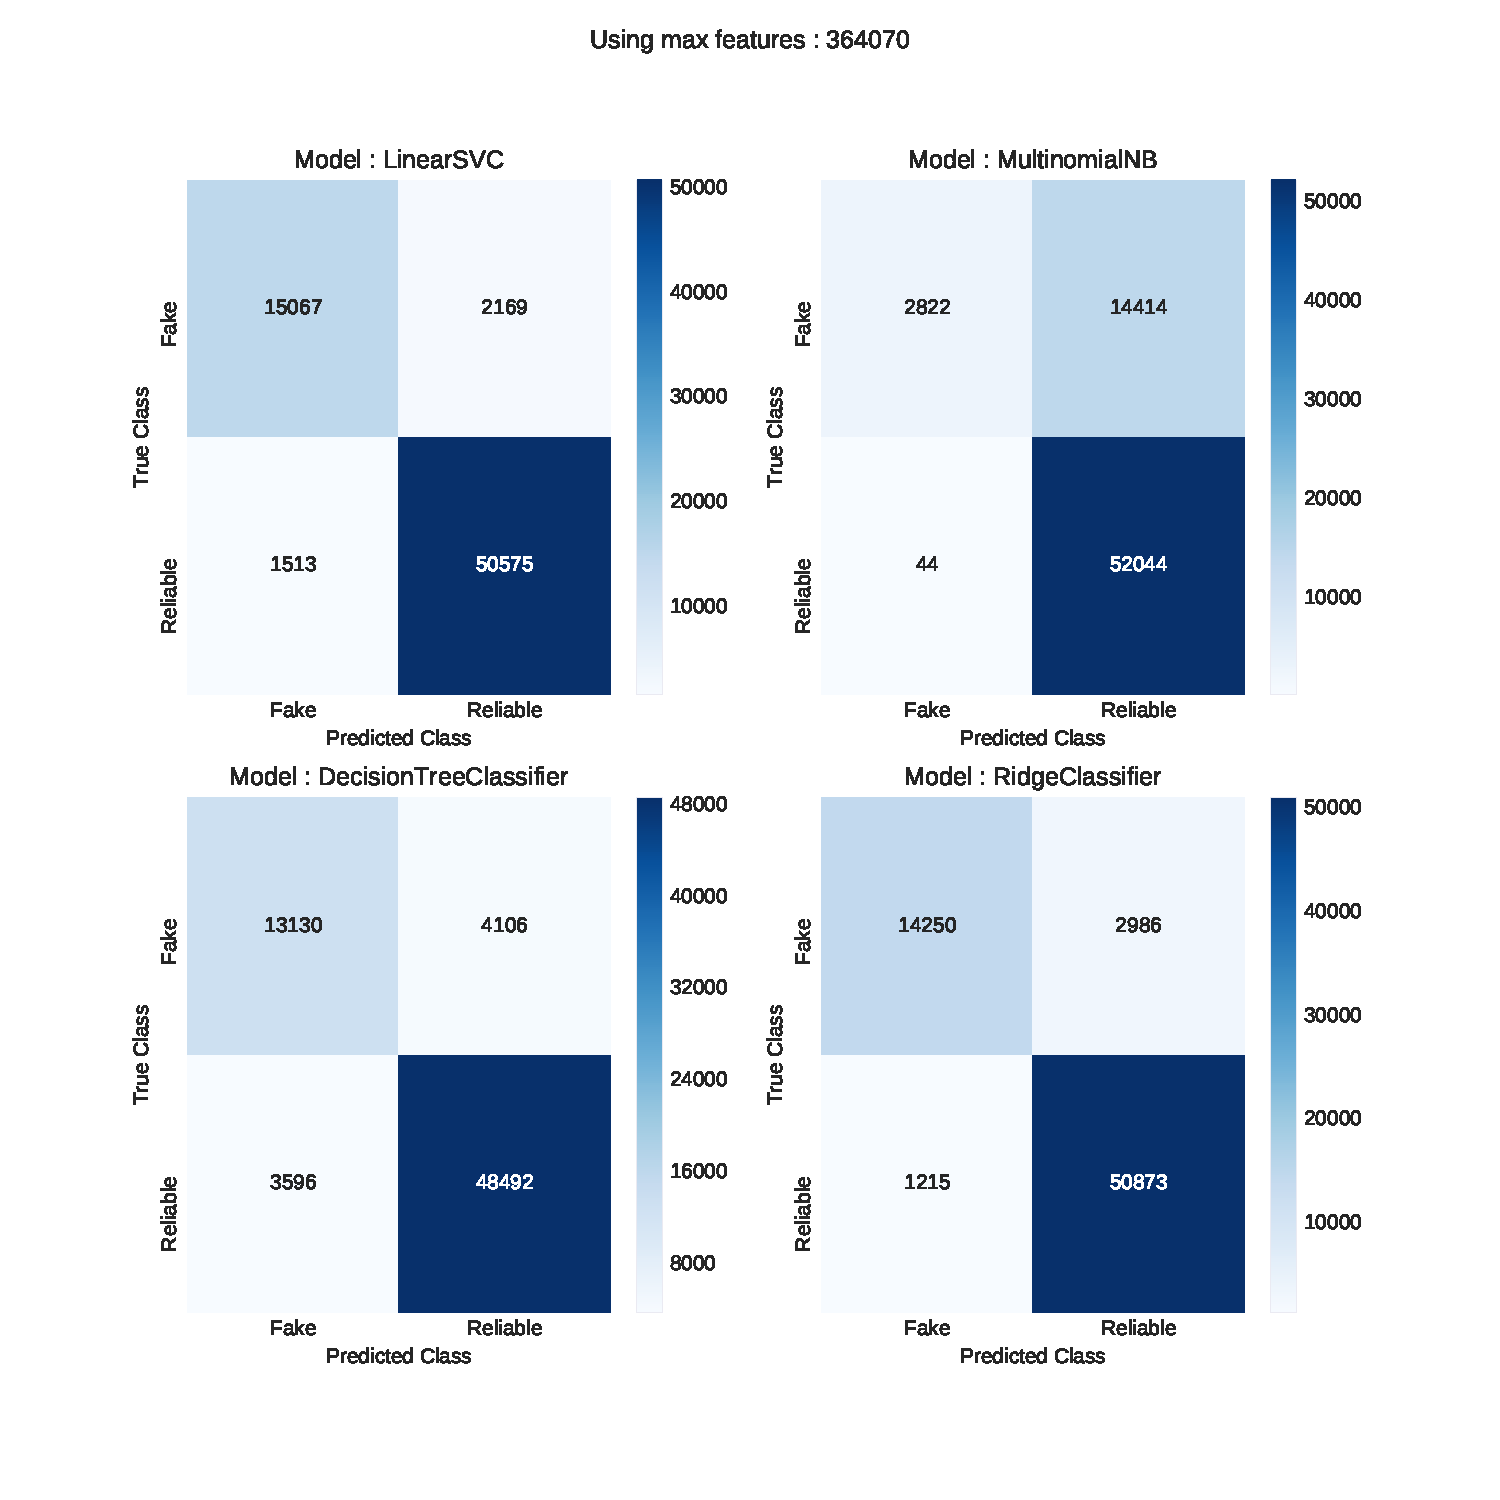
\includegraphics[width=0.8\textwidth]{images/chapitre3/confMat_fake_364070}
	\caption{Confusion matrix for each model using $364,070$ features}
	\label{fig:chap3:confMat1}
\end{figure*}